\documentclass{article}
% PAGE PROPERTIES
\usepackage[margin=0.75in]{geometry}
\usepackage{pdflscape}

% FONT
\usepackage[LGR,T1]{fontenc}
\usepackage{hyperref}
\hypersetup{
    colorlinks,
    linkcolor={red},
    citecolor={orange},
    urlcolor={blue!80!black}
}

% GRAPHICS
\usepackage{graphicx}
\usepackage{tikz}
\usepackage{pgfplots}
\usetikzlibrary{angles,
                graphs,
                graphs.standard, 
                quantikz2, 
                decorations.pathmorphing,
                patterns, 
                patterns.meta,
                shadows,
                shapes.geometric,
                positioning}
\tikzset{snake it/.style={decorate, decoration=snake}}
\pgfplotsset{compat=1.18} 
% MATHEMATICAL
\usepackage{physics}
\usepackage{amsmath,amsfonts}
\usepackage{amssymb}

% CODE
\usepackage{csvsimple}
\usepackage{listings}
\usepackage{minted}

% LISTS and TABLES
\usepackage{paralist}
\usepackage{multirow}


% BOXES and FRAMES
\usepackage{mdframed}
    \newmdtheoremenv{defn}{Definition}
    \newmdtheoremenv{thrm}{Theorem}
    \newmdtheoremenv{thrm*}{Theorem}
    \newmdtheoremenv{hlo}{Overview}
    \newmdtheoremenv{lmma}{Lemma}
    \newmdtheoremenv{prop}{Proposition}
% USEFUL MATH COMMANDS
\newcommand{\ci}{\mathrm{i}}
\newcommand{\ce}{\mathrm{e}}
\newcommand{\bin}[1]{\mathtt{#1}}
\DeclareMathAlphabet{\mathgtt}{LGR}{cmtt}{m}{n}
\usepackage[margin=3cm]{caption}
\usepackage[greek,english]{babel}
\tikzset{every picture/.style={/utils/exec={\ttfamily}}}
\usepackage{tikz,tikz-3dplot}
\usepackage{tikz-3dplot-circleofsphere}
\usetikzlibrary{shadings,intersections}

\usepackage{setspace}
\doublespacing

\title{\textsc{\textbf{Report:}}\\ Hamiltonian Simulation via \\ Quantum Signal Processing}
\author{Gabriel Waite}
\date{August 2023}

\begin{document}

\maketitle

\section{Introduction}
The manipulation of matrices is key to progressing quantum algorithms, specifically in crafting matrix functions. Fluidly performing various operations efficiently is essential to creating a true quantum advantage in the algorithm space. At the heart of matrix functions and arguably underpinning the idea of quantum computation \cite{Feynman82} is the concept of Hamiltonian simulation. Physics 101 teaches the famous Schrödinger equation --- the basis for Hamiltonian simulation,
\begin{equation}\label{eq:shcrodinger_eq}
    H\ket{\psi(t)} = -i\pdv{t}\ket{\psi(t)}
\end{equation}
The idea in quantum computation is to simulate the evolution of this system by implementing the matrix exponential,
\begin{equation}\label{eq:exp_H}
    \ce^{\ci Ht}
\end{equation}
Such a simple expression has produced a vast array of research and techniques aimed at giving efficient simulation. It was proven by Lloyd \cite{Lloyd1996} that indeed, quantum computers can be used to simulate the dynamics of local Hamiltonians. The justification for considering local Hamiltonians was due to the fact systems in nature exhibit such properties \cite{Ambainis14QMA,CN14}. The primitive method employed by Lloyd was related to the Trotter--Suzuki--Lie method, which decomposes the matrix exponential into smaller steps,
\begin{equation}
    \ce^{\ci Ht} = \big(\ce^{\ci H_1 \frac{t}{n} + \ldots + \ci H_m \frac{t}{n}} \big)^n = \big(\ce^{\ci H_1 \frac{t}{n}}\ldots \ce^{\ci H_m \frac{t}{n}} + \mathcal{E} \big)^n
\end{equation}
where $\norm{\mathcal{E}} = O(m^2t^2/n^2)$. By choosing a sufficient value for $n$, it can be shown that $U = \big(\ce^{\ci H_1 \frac{t}{n}}\ldots \ce^{\ci H_m \frac{t}{n}}\big)^n$ approximates eq. (\ref{eq:exp_H}) within some error $\varepsilon$. Notice with this method that the number of gates needed scales quadratically with time, while efficient from a theoretical computer science perspective, is not realistically ideal for long time intervals!

The goal of Hamiltonian simulation is to produce an efficient simulation of the matrix exponential of some Hamiltonian up to a defined error, specifically, construct some $U$ such that,
\begin{equation}\label{eq:expH_norm}
    \norm{U - \ce^{\ci Ht}} \leq \varepsilon
\end{equation}
In this essay, we analyse pieces of a new approach for Hamiltonian simulation --- \emph{quantum signal processing} (\textsc{qsp}) \cite{LC17}; specifically the single ancilla variant. Before delving into this idea, however, we must fulfil some prerequisites. Below, fig. \ref{fig:pipeline}, shows a workflow of concepts that lead ultimately to another technique, the quantum singular value transformation \cite{GSLW19}. We do not cover that here; however, we do note that this technique is a further generalisation of \textsc{qsp} (and other ideas); it is a powerful concept that has arguably led to the idea of a `grand unification' of quantum algorithms \cite{MRTC21}.

\begin{figure}[h!]
    \centering
    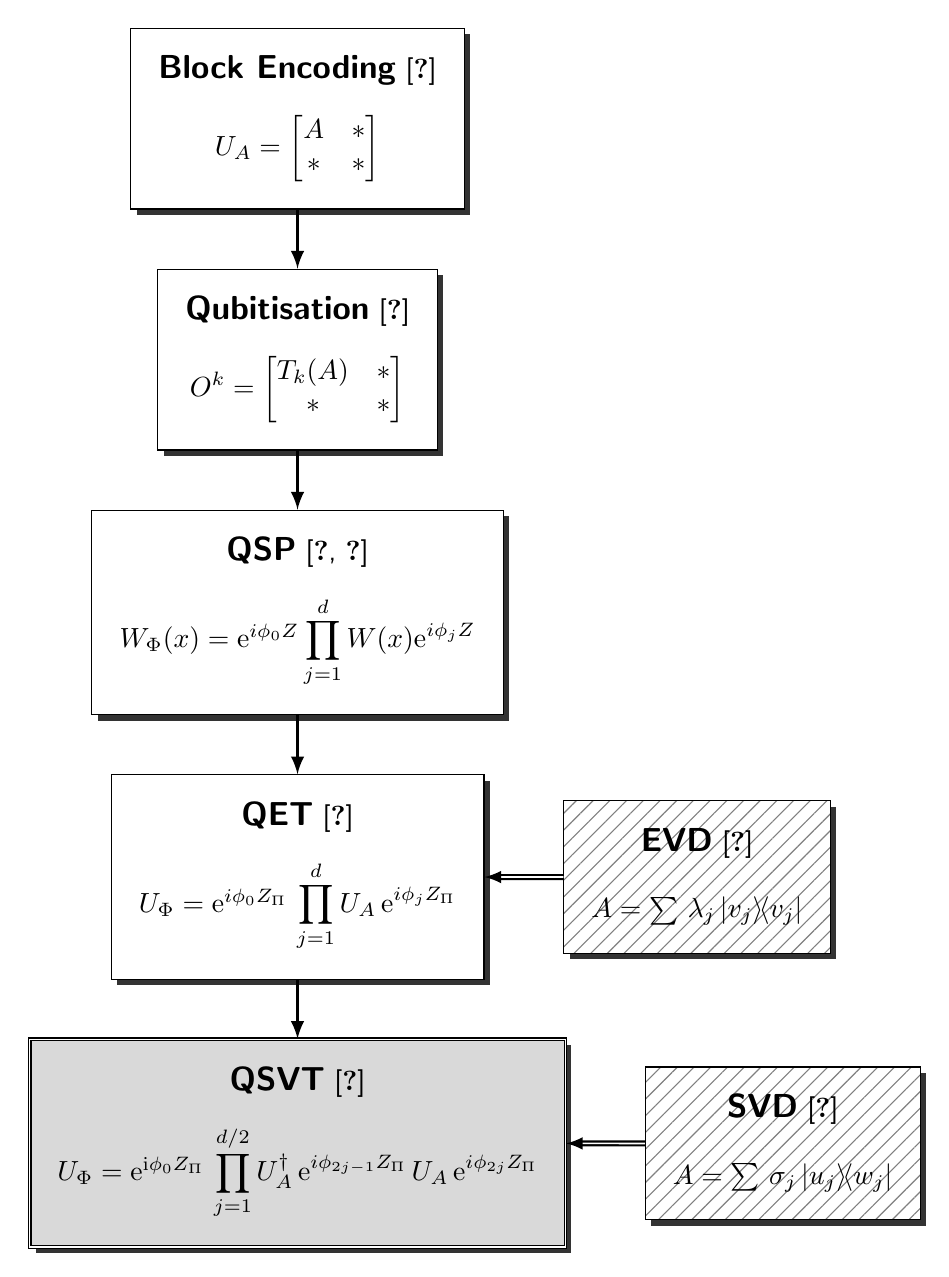
\begin{tikzpicture}[
        node distance=7.5mm and 10mm,
    box/.style = {draw, minimum height=15mm, inner xsep=3mm, inner sep=10pt, align=center},
    every shadow/.style={opacity=.8,fill=black},
    every edge quotes/.style = {align=center},
         font = \sffamily,
         scale=0.8
                            ]
    \node[drop shadow, fill=white] (n1) [box]             {{\large\textbf{Block Encoding}} \cite{LinLin22}\\~\\$U_A = \begin{bmatrix}A & * \\ * & *\end{bmatrix}$};
    \node[drop shadow, fill=white] (n2) [box,below=of n1] {{\large\textbf{Qubitisation}} \cite{LC19}\\~\\$O^k = \begin{bmatrix}T_k(A)&*\\ *&*\end{bmatrix}$};
    \node[drop shadow, fill=white] (n3) [box,below=of n2] {{\large\textbf{QSP}} \cite{LYC16,LC19}\\~\\$W_\Phi(x) = \ce^{i\phi_0Z}\displaystyle\prod_{j=1}^d W(x)\ce^{i\phi_jZ}$};
    \node[drop shadow, fill=white] (n4) [box,below=of n3] {{\large\textbf{QET}} \cite{DT22}\\~\\$U_{\Phi} = \ce^{i\phi_0 Z_{\Pi}}\,\displaystyle\prod_{j=1}^d U_A\,\ce^{i\phi_jZ_\Pi}$};
    \node[double, fill=white!85!black, drop shadow] (n5) [box,below=of n4] {{\large\textbf{QSVT}} \cite{GSLW19}\\~\\ $U_{\Phi} = \ce^{\ci\phi_0  Z_{\Pi}}\,\displaystyle\prod^{d/2}_{j=1} U_A^\dagger\,\ce^{i\phi_{2j-1} Z_\Pi}\,U_A \,\ce^{i\phi_{2j} Z_\Pi}$};
    \node[drop shadow, fill=white,pattern={Lines[
                  distance=1.5mm,
                  angle=45,
                  ]}, pattern color=gray,preaction={fill=white}] (n6) [box,right=of n4] {{\large\textbf{EVD}} \cite{Serre02}\\~\\$A=\sum\,\lambda_j\ketbra{v_j}{v_j}$};
    \node[drop shadow, fill=white,pattern={Lines[
                  distance=1.5mm,
                  angle=45,
                  ]}, pattern color=gray,preaction={fill=white}] (n7) [box,right=of n5] {{\large\textbf{SVD}} \cite{Serre02}\\~\\$A=\sum\,\sigma_j\ketbra{u_j}{w_j}$};
    
    
    \draw[very thick,-latex](n1) -- (n2);
    \draw[very thick,-latex](n2) -- (n3);
    \draw[very thick,-latex](n3) -- (n4);
    \draw[very thick,-latex](n4) -- (n5);
    \draw[thick,double,-latex](n6) -- (n4);
    \draw[thick,double,-latex](n7) -- (n5);
    
    \end{tikzpicture}
    \caption{Pipeline of quantum techniques that build from block encoding. Block encoding supports the notion of quantum signal processing, which in turn can be generalised via the quantum eigenvalue transformation. The quantum eigenvalue transformation can be further generalised to the quantum singular value transformation. The final two techniques can be understood as quantum analogous to the robust mathematical concepts of eigenvalue decomposition and singular value decomposition, respectively.}
    \label{fig:pipeline}
\end{figure}

\clearpage
\section{Block Encoding}
The idea of block encoding can be described succinctly as a technique that allows for the application of some general matrix $A\in\mathbb{C}^{2^n\times 2^n}$, where $A$ is not necessarily unitary, on a quantum state. A requirement for quantum gates implemented on a quantum circuit is unitarity; however, one may be interested in the dynamics of a state under the influence of a non--unitary matrix. Block encoding, therefore, answers the question: \emph{how could we implement $A$ on a quantum computer}?

At a basic level, the technique embeds $A$ within some larger but unitary matrix to allow for its implementation on a quantum computer. A trivial example: the \textsc{cnot} gate, which encodes the action of the Pauli--$X$ gate on some target qubit(s), dictated by the state of the control qubit(s). Block encoding is slightly more general than this; however, the intuition is analogous, cf. Fig. \ref{fig:BE_diagram}.

\begin{figure}[h!]
    \centering
    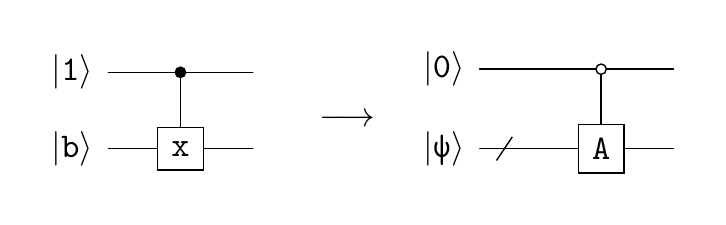
\begin{tikzpicture}
        \node[scale=1.25]{
    \begin{quantikz}[thin lines]
        \lstick{$\mathtt{\ket{1}}$}&\ctrl{1}&\qw\\
        \lstick{$\mathtt{\ket{\text{b}}}$}&\gate{\mathtt{x}}&\qw                   
    \end{quantikz}
    $\quad\longrightarrow\quad $\begin{quantikz}[thin lines]
        \lstick{$\mathtt{\ket{0}}$}&\qw&\octrl{1}&\qw\\
        \lstick{$\ket{\text{\textgreek{ψ}}}$}&\qwbundle{}&\gate{\mathtt{A}}&\qw     
    \end{quantikz}
        };
    \end{tikzpicture}
    \caption{(Right) A trivial example of a block encoded insatnce ---  the \textsc{cnot} gate that performs $\ket{b}\mapsto\ket{b\oplus 1}$ upon signal state $\ket{1}$ on the first register. (Left) A generalised block encoding circuit, triggered when the signal state is $\ket{0}$ (eq. (\ref{eq:BE})).}
    \label{fig:BE_diagram}
\end{figure}

Assuming this larger unitary $U_A\in\mathbb{C}^{2^\eta\times 2^\eta}$ exists, where $\eta = n+m$ and the state $\ket{0^m,\psi}$ can be efficiently prepared, then,
\begin{equation}\label{eq:BE}
    U_A = \begin{bmatrix}A & * \\ * & *\end{bmatrix}
\end{equation}
block encodes the activity of $A$ onto the state $\ket{\psi}$. The matrix components marked `$*$' are not important for introductory purposes, and so will not be specified but exist in a manner such that $U_A$ is unitary. The action of $U_A$ on $\ket{0^m,\psi}$ can trivially be found as,
\begin{equation}\label{eq:BE_states}
    U_A\ket{0^m,\psi} = \ket{0^m}A\ket{\psi} + \ket{\perp}
\end{equation}
Additionally, the state $\ket{\perp}$ remains unspecified but is orthogonal with respect to $\ket{0^m}\otimes \mathbb{I}_n$. One subtle condition for the existence of $U_A$ is $\norm{A}\leq 1$ \cite{CLBY23}. If, for instance, $\norm{A}>1$, we can just renormalise via a block encoding of $A/\alpha$, such that $\norm{A/\alpha}\leq 1$. Notice that the outcome we desire, i.e. the effect, $A\ket{\psi}$, can be found by a measurement on the first register, see fig. \ref{fig:BE_A}. The probability of success is, then,
\begin{equation}
    \mathcal{P}(\ket{0^m}) = \frac{\norm{A\ket{\psi}}^2}{\alpha^2}
\end{equation}
With $O\big(1/\sqrt{\mathcal{P}(\ket{0^m})}\big)$ round of amplitude amplification, we can boost the probability of success. A very general definition can be given for the block encoding of a matrix. Note that the explicit form of a block encoding need not take the exact form shown in eq. (\ref{eq:BE}) and in fact the action of $A$ can be extracted from the encoding $U_A$ via some \emph{signal state} $\ket{G}$. Moreover,
\begin{defn}{\textnormal{\cite{LinLin22,LC19}}}

    \noindent Given an $n$-qubit matrix $A$, if we can find parameters, $\alpha, \epsilon \in \mathbb{R}^+$ and an $(m+n)$-qubit unitary, $U_A$, and a signal state $\ket{G}\in\mathbb{C}^{2^m}$, such that, 
    \begin{equation}
    \norm{A - \alpha \left(\bra{G}\otimes\mathbb{I}_n\right)U_A\left(\ket{G}\otimes\mathbb{I}_n\right)} \leq \epsilon
    \end{equation}
    Then $U_A$ is the $(\alpha, m, \epsilon)$--\textsc{be} of $A$.
\end{defn}

Notice that the circuit shown in fig. \ref{fig:BE_A} can be repeated several times to generate powers of $A$. This probes the idea of block encoding functions of matrices, i.e. $f(A)$. This is the basis for \emph{qubitisation} \cite{LC19}; qubitisation uses a block encoded iterate in the eigenbasis of a Hamiltonian to craft Chebyshev polynomials on said Hamiltonian. The term qubitisation refers to the 2D space spanned by the states, reminiscent of eq. (\ref{eq:BE_states}).

It turns out not all possible functions can be constructed exactly; using truncated Taylor expansions, decent approximations can be found. Block encoding strongly overlaps with a technique known as `linear combination of unitaries' \cite{CW12}. A simple example of such would be the block encoding of $A + B$ via the \textsc{LCU} method. Figure \ref{fig:LCU} gives the circuit diagram for such. A quick calculation shows that measuring $\ket{0}$ on the first register produces $(A+B)\ket{\psi}$. Clearly, if $B=A^2$, the function $f(x)=x(1+x)$ is trivially constructable. By having a longer combination of such unitaries, it is straightforward to see how a truncated series expansion can be implemented.

\begin{figure}[h!]
    \centering
    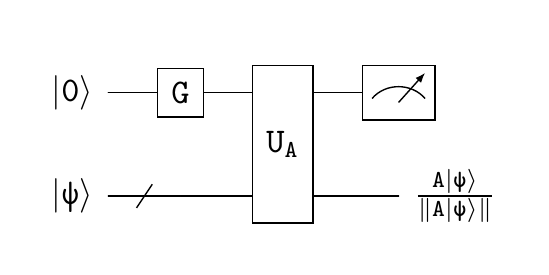
\begin{tikzpicture}
        \node[scale=1.25]{
    \begin{quantikz}[thin lines]
        \lstick{$\mathtt{\ket{0}}$}&\gate{\mathtt{G}}&\gate[2]{\mathtt{U_A}}&\meter{} \\
        \lstick{$\mathtt{\ket{\text{\textgreek{ψ}}}}$}&\qwbundle{}&                      &\qw\rstick{$\mathtt{\frac{A\ket{\text{\textgreek{ψ}}}}{\norm{A\ket{\text{\textgreek{ψ}}}}}}$}
    \end{quantikz}
        };
    \end{tikzpicture}
    \caption{Block encoding of a matrix $A$ with signal state $\ket{G} = G\ket{0}$.}
    \label{fig:BE_A}
\end{figure}

\begin{figure}[h!]
    \centering
    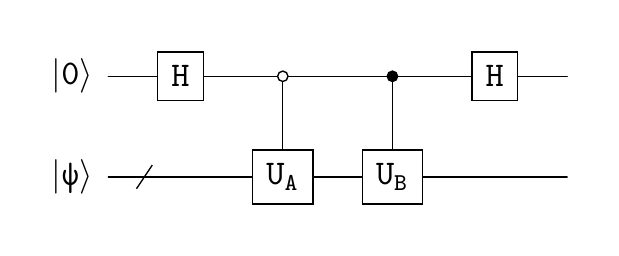
\begin{tikzpicture}
        \node[scale=1.25]{
    \begin{quantikz}[thin lines]
        \lstick{$\ket{\mathtt{0}}$} &\gate{\mathtt{H}}&\octrl{1}          &\ctrl{1}           &\gate{\mathtt{H}}&\qw \\
        \lstick{$\ket{\text{\textgreek{ψ}}}$}          &\qwbundle{}              &\gate{\mathtt{U_A}}&\gate{\mathtt{U_B}}&\qw&\qw
    \end{quantikz}
        };
    \end{tikzpicture}
    \caption{An instance of the linear combination of unitaries technique that encodes the action of $A+B$ on the state $\ket{\psi}$.}
    \label{fig:LCU}
\end{figure}

There are some apparent bottlenecks to this method. The definition above emphasises the existence of the signal state $\ket{G}$, and more generally, the block encoding of $A$ usually comes in the form of constructing oracles that can efficiently query the elements \cite{BCK15,CKS17}. For specific examples of sparse matrices, such oracles have been explicitly calculated \cite{CLBY23}. 

\clearpage
\section{Single Qubit Rotations}
Before an analysis of the quantum signal processing technique, let us briefly discuss the action of a simple single qubit rotation gate --- the rotation--$X$ gate,
\begin{equation}\label{eq:rotX}
    R_{\textsc{x}}(\theta) = \ce^{-\ci \theta X} = \cos\frac{\theta}{2}\mathbb{I} - \ci\sin\frac{\theta}{2}X
\end{equation}
Clearly, this just rotates a state around the $\ket{+}/\ket{-}$ axis of the Bloch sphere. Note that all pure states can be geometrically represented on the boundary of the Bloch sphere, $S^2 = \partial B^3$, via,
\begin{equation}
    \ket{\psi} = \cos\frac{\theta}{2}\ket{0} + \ce^{\ci \phi}\sin\frac{\theta}{2}\ket{1}
\end{equation}
where $\theta$ describes a rotation about the $\ket{+}/\ket{-}$ axis and $\phi$ a rotation about the $\ket{0}/\ket{1}$ axis\footnote{It is common for $\theta$ and $\phi$ to be referred to as the polar and azimuthal angle respectively}. To a get a more intuitive picture of $R_{\textsc{x}}$'s effect, imagine rotating the $\ket{0}$ state by some angle $\theta$ --- it then becomes a superposition of $\ket{0}$ and $\ket{1}$. The addition of the $\phi$ allows for further rotation along the line of latitude at which the state lies. We would find that all pure states conform to following a circular path under a sequence of $R_{\textsc{x}}$ rotations; fig. \ref{fig:rx_examples} shows some examples of the effect of sequential $R_{\textsc{x}}$ applications. 

\begin{figure}[h!]
    \centering
        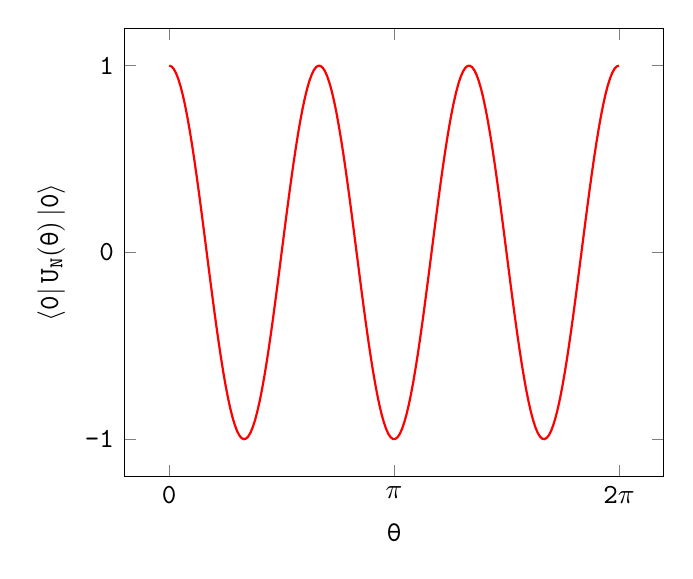
\begin{tikzpicture}
            \begin{axis}[
            domain=0:2*pi,
            xtick={0,pi,2*pi},
            xticklabels={0,$\mathtt{\pi}$,$\mathtt{2\pi}$},
            xlabel={\textgreek{\ttfamily θ}},
            ytick={-1,0,1},
            yticklabels={-1,0,1},
            ylabel={$\mathtt{\bra{0}U_N(\text{\textgreek{θ}})\ket{0}}$}
        ]
            \addplot[samples=200,mark=none,thick, red] {cos(deg(3*x))}; 
            \end{axis}
        \end{tikzpicture}
    \caption{Graphical representation of the function traced by a pure state after a series of $R_{\textsc{x}}(\theta)$ rotations}
    \label{fig:cos}
\end{figure}

More formally, let $U_N(\theta) = R_{\textsc{x}}(\theta)\ldots R_{\textsc{x}}(\theta)$ which is generated by $N$ applications of the rotation--$X$ gate. This produces $f(x)=\cos \frac{Nx}{2}$ in the upper right corner of $U_N(\theta)$ and hence,
\begin{equation}
    \bra{0}U_N(\theta)\ket{0} = \cos\frac{N\theta}{2}
\end{equation}
The plots of fig. \ref{fig:rx_examples} correlate with the result shown in fig. \ref{fig:cos}! It is easy to conclude that $U_N(\theta)$ can only give circular paths on $\partial B^3$. An important question: \emph{how do we impart more control on the system}? This is the basis argument for the \textsc{qsp} technique. By conjugating $R_{\textsc{x}}(\theta)$ with $R_{\textsc{z}}(\phi) = \ce^{\ci \phi Z/2}$ gates we can perform more complex actions!

\begin{figure}[h!]
    \centering
    \def\r{1.5}
    \tdplotsetmaincoords{60}{125}
    \begin{tikzpicture}[tdplot_main_coords,scale=1.3]
        \begin{scope}[thin,black!30]
        \draw[->] (0,-1.3*\r,0) -- (0,1.3*\r,0);
        \draw[tdplot_screen_coords] (0,0,0) circle (\r);
        \tdplotCsDrawLatCircle{\r}{0}
        \draw[-latex,red, thick] (0,0,0)--(0,1.65,1.3);
        \tdplotsetthetaplanecoords{0}
        \tdplotdrawarc[tdplot_rotated_coords,->,color=black]{(0,0,0.5)}{0.2}{110}{460}{anchor=south west,color=black}{}
        \end{scope}
        \tdplotCsDrawCircle{\r}{90}{90}{35}
    \end{tikzpicture}
    \hspace{1cm}
    \begin{tikzpicture}[tdplot_main_coords,scale=1.3]
        \begin{scope}[thin,black!30]
        \draw[->] (0,-1.3*\r,0) -- (0,1.3*\r,0);
        \draw[tdplot_screen_coords] (0,0,0) circle (\r);
        \tdplotCsDrawLatCircle{\r}{0}
        \draw[-latex,red, thick] (0,0,0)--(0,0,\r);
        \tdplotsetthetaplanecoords{0}
        \tdplotdrawarc[tdplot_rotated_coords,->,color=black]{(0,0,0.5)}{0.2}{110}{460}{anchor=south west,color=black}{}
        \end{scope}
        \tdplotCsDrawCircle{\r}{-90}{90}{0}
    \end{tikzpicture}
    \hspace{1cm}
    \begin{tikzpicture}[tdplot_main_coords,scale=1.3]
        \begin{scope}[thin,black!30]
        \draw[->] (0,-1.3*\r,0) -- (0,1.3*\r,0);
        \draw[tdplot_screen_coords] (0,0,0) circle (\r);
        \tdplotCsDrawLatCircle{\r}{0}
        \end{scope}
        \tdplotCsDrawCircle{\r}{-90}{90}{55}
        \draw[-latex,red, thick] (0,0,0)--(0,-0.63,0.63);
        \tdplotsetthetaplanecoords{0}
        \tdplotdrawarc[tdplot_rotated_coords,->,color=black]{(0,0,0.5)}{0.2}{110}{460}{anchor=south west,color=black}{}
    \end{tikzpicture}
    \caption{A series of different pure state vectors lying on the surface of the Bloch sphere, $\partial B^3$, undergoing a sequence of $R_{\textsc{x}}$ rotations. The path ultimately traced out by each is a circular one (given a large enough sequence).}
    \label{fig:rx_examples}
\end{figure}

\clearpage
\section{Quantum Signal Processing}
Consider the following single qubit rotation gate,
\begin{equation}
    R_\phi(\theta) = \exp\big(-\ci \frac{\theta}{2}(\cos\phi X + \sin\phi Y)\big)
\end{equation}
Using spectral decomposition, we can express this unitary as,
\begin{equation}
    R_\phi(\theta) = \ce^{-\ci\frac{\theta}{2}}\ketbra{\eta_+} + \ce^{\ci\frac{\theta}{2}}\ketbra{\eta_-}
\end{equation}
Where $\ket{\eta_\pm} \sim \ket{0} \pm \ce^{\ci \phi}\ket{1}$. In this manner, we can easily translate the gate into its matrix form as follows,
\begin{equation}\label{eq:raw_ctrlrot}
    R_\phi(\theta) = \begin{bmatrix}
                        \cos\theta/2 & -\ci \ce^{-\ci\phi}\sin\theta/2 \\
                        -\ci \ce^{\ci\phi}\sin\theta/2 & \cos\theta/2
                     \end{bmatrix}
\end{equation}
When in this form, the identification $R_\phi(\theta) = R_{\textsc{z}}(-\phi + 2\pi)R_{\textsc{x}}(\theta) R_{\textsc{z}}(\phi + 2\pi)$ can be made with a simple calculation and thus the extra control can easily be seen via the presence of $\phi$ terms! Informally, a sequence of $R_\phi(\theta)$ operations can produce specific polynomials (beyond $\cos x$), figs. \ref{fig:phi_graph1},\ref{fig:phi_graph2} provide insight into possible functions achievable and $\partial B^3$ paths. 

\begin{figure}[h!]
    \centering
    \begin{tikzpicture}[scale=1.2]
        \begin{axis}[
            xtick={0,pi,2*pi},
            xticklabels={0,$\mathtt{\pi}$,$\mathtt{2\pi}$},
            xlabel={\textgreek{\ttfamily θ}},
            ytick={-1,0,1},
            yticklabels={-1,0,1},
            ylabel={Re$\big[\mathtt{\bra{0}R_{\text{\textgreek{\ttfamily φ}}_{N}}(\text{\textgreek{\ttfamily θ}})\ldots R_{\text{\textgreek{\ttfamily φ}}_{1}}(\text{\textgreek{\ttfamily θ}})\ket{0}}\big]$}
        ]
            \addplot[color=blue,thick] table [y=freq,x=theta,mark=none]{VariedPhiGraph1.txt};
            \addplot[color=red,thick] table [y=freq,x=theta,mark=none] {VariedPhiGraph2Alt.txt};
            \addplot[color=orange,thick] table [y=freq,x=theta,mark=none]{VariedPhiGraph4Alt.txt};
            \addplot[color=magenta,thick] table [y=freq,x=theta,mark=none]{VariedPhiGraph4.txt};
        \end{axis}
    \end{tikzpicture}
    \caption{Graphical representation of possible functions constructable via a series of $R_\phi(\theta)$ applications according to different random $\boldsymbol{\Phi}\in\mathbb{R}^N$}
    \label{fig:phi_graph1}
\end{figure}

\begin{figure}[h!]
    \centering
    \def\r{1.5}
    \tdplotsetmaincoords{60}{125}
    \begin{tikzpicture}[tdplot_main_coords,scale=1.3]
        \begin{scope}[thin,black!30]
        \draw[->] (0,-1.3*\r,0) -- (0,1.3*\r,0);
        \draw[tdplot_screen_coords] (0,0,0) circle (\r);
        \tdplotCsDrawLatCircle{\r}{0};
        \draw[-latex,red, thick] (0,0,0)--(0,1.65,1.3);
        \tdplotsetthetaplanecoords{0};
        \tdplotdrawarc[tdplot_rotated_coords,->,thin,black!50]{(0,0,0.5)}{0.2}{110}{460}{anchor=south west,color=black}{};
        \end{scope}
        \draw [black] plot [smooth] coordinates {
        (0,1.63,1.3)
        (0,1.1,1.4)
        (0,0.7,1.1)
        (0,0.6,0.4)
        (0,0.1,-0.3)
        (0,0.1,-0.8)
        (0,0,-1.4)
        (0,0.4,-1.47)
        (0,0.6,-1.4)
        (0,0.8,-1.28)};
        \draw [black,dashed] plot [smooth] coordinates {
        (0,1.63,1.3)
        (0,1.65,1.)
        (0,1.6,0.8)
        (0,1.65,0.4)
        (0,1.65,0)
        (0,1.3,-0.5)
        (0,0.8,-1)
        (0,0.8,-1.28)};
    \end{tikzpicture}
    \caption{A possible path taken by a vector on $\partial B^3$ after a sequence of $R_\phi(\theta)$}
    \label{fig:phi_graph2}
\end{figure}


The sequence of $R_\phi(\theta)$'s can be expanded into the Pauli basis such that each Pauli matrix is coupled with some real function. This is the main idea of \textsc{qsp} --- to craft approximations to generic functions using simple rotation gates. The decomposition follows \cite{LYC16,LC19},
\begin{equation}
    V_{\boldsymbol{\Phi}}(\theta) = A(\theta)\mathbb{I} + \ci B(\theta)Z + \ci C(\theta)X + \ci D(\theta)Y
\end{equation}
where $A(\theta),B(\theta),C(\theta),D(\theta)$ are real and $\boldsymbol{\Phi}\in\mathbb{R}^N$. A neat trick finds that not all functions need to be evaluated, and we can reduce our study to just $A,C$ \cite{LC19}. This gives insight into the particular state we desire for the ancilla. Specifically, $\bra{+}V_{\boldsymbol{\Phi}}(\theta)\ket{+} = A(\theta) + \ci C(\theta)$. We now state the theorem underpinning the capabilities of the single ancilla \textsc{qsp} method:

\begin{thrm}{\textnormal{\cite{LC17,LC19}}}\label{thrm:1}
    
    \noindent For any even $N>0$ and a choice of real functions, $A(\theta)$, $C(\theta)$, can be implemented by a set of angles, $\boldsymbol{\Phi}\in\mathbb{R}^N$, if and only if:
    \begin{enumerate}[(i)]
        \item $\forall \theta \in \mathbb{R}$, $A^2(\theta) + C^2(\theta)\leq 1$
        \item $A(0) = 1$
        \item $A(\theta) =\displaystyle\sum_{k=0}^{N/2} a_k \cos(k \theta)$ gives a real cosine Fourier series of degree at most $N/2$
        \item $C(\theta) =\displaystyle\sum_{k=0}^{N/2} c_k \sin(k \theta)$ gives a real sine Fourier series of degree at most $N/2$
    \end{enumerate}
\end{thrm}

Given the above theorem and ideas, the \textsc{qsp} technique is aimed at implementing the following transformation,
\begin{equation}\label{eq:v_ideal}
    V = \sum_\lambda \ce^{\ci h(\lambda)}\ketbra{\lambda}
\end{equation}
where $\ket{\lambda}$ are the eigenvectors of some unitary $W$; moreover,
\begin{equation}
    W\ket{\lambda} = \ce^{\ci \lambda}\ket{\lambda}
\end{equation}
The circuit for $V$ transforms the eigenphases of $\ket{\lambda}$ according to the real function $h(x)$, created using a sequence of $R_\phi(\theta)$ gates. Ideally, $V$ uses minimal queries to $W$. In circuit diagram language, $V$ is a sequence of unitary rotation gates, $U_{\phi_j}$, shown in fig. \ref{fig:v_ideal}. 

\begin{figure}[h!]
    \centering
    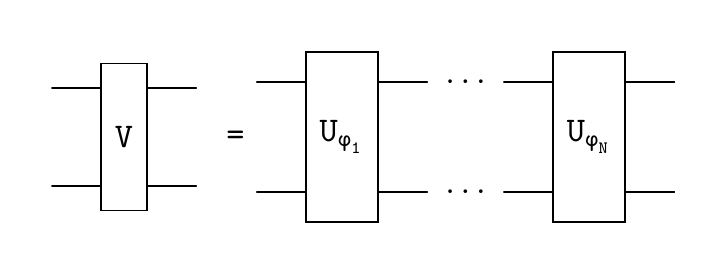
\begin{tikzpicture}
        \node[scale=1.25]{
    \begin{quantikz}[thin lines]
        \qw&\gate[2]{\mathtt{V}}&\qw \\
        \qw& &\qw
    \end{quantikz}
    =\begin{quantikz}[thin lines]
        \qw&\gate[2]{\mathtt{U_{{\text{\textgreek{\ttfamily φ}}}_1}}}&\qw \ \ldots \ &\gate[2]{\mathtt{U_{{\text{\textgreek{\ttfamily φ}}}_N}}}&\qw \\
        \qw&                                                       &\qw \ \ldots \ & &\qw
    \end{quantikz}
        };
    \end{tikzpicture}
    \caption{The sequence of $U_{\phi}$ gates applied to produce the ideal unitary $V$ which transforms the eigenphases accoring to some real function $h(x)$.}
    \label{fig:v_ideal}
\end{figure}

The individual $U_{\phi}$ are related to $R_\phi(\theta)$ and a controlled--$W$ gate. The exact form of $U_{\phi}$ can be defined as,
\begin{equation}\label{eq:u_phi}
    U_{\phi} = \sum_\lambda R_\phi(\lambda)\otimes \ketbra{\lambda}
\end{equation}
With a little bit of work, it can be shown that the circuit diagram of fig. \ref{fig:u_phi} is sufficient for implementing $U_{\phi}$

\begin{figure}[h!]
    \centering
    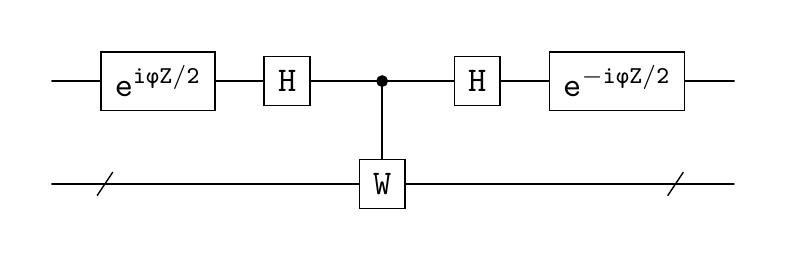
\begin{tikzpicture}
        \node[scale=1.25]{
    \begin{quantikz}[thin lines]
        \qw&\gate{\mathtt{e^{i \text{\textgreek{\ttfamily φ}} Z/2}}}&\gate{\mathtt{H}}&\ctrl{1}         &\gate{\mathtt{H}}&\gate{\mathtt{e^{-i \text{\textgreek{\ttfamily φ}} Z/2}}}&\qw\\
        \qw&\qwbundle{}                                  &\qw              &\gate{\mathtt{W}}&\qw              &\qw                                   &\qwbundle{}
    \end{quantikz}
        };
    \end{tikzpicture}
    \caption{A circuit diagram showing how to construct $U_{\phi}$ using a single controlled--$W$ gate and $O(1)$ other single qubit rotation gates.}
    \label{fig:u_phi}
\end{figure}

Notice an eigenstate input renders $U_{\phi}$ as $R_\phi(\lambda)$! In this regard, it can be shown,
\begin{equation}
    V = \bigoplus_{\lambda} \left(\ce^{\ci\varphi_0 Z} \left(\prod_{j=1}^N R_{\textsc{x}}(
    \lambda)\ce^{\ci\varphi_j Z} \right) \right)\otimes\ketbra{\lambda} = \begin{bmatrix}f[W] & * \\ * & *\end{bmatrix}
\end{equation}


By selecting a specific $\boldsymbol{\Phi}$, an approximation to $\ce^{\ci h(\lambda)}$ can be implemented according to the rules of Theorem \ref{thrm:1}. Principally, this is what quantum signal processing does, with $O(N)$ queries to $W$ and post--selecting the $\ket{+}$ state on the ancilla qubit. The addition of a single ancilla allows for opposing parity on $A$ and $C$, whereas the no--ancilla variant \cite{LC19} renders both functions having like parity. In this regard, the single ancilla variant has more freedom. 

\clearpage
\section{Hamiltonian Simulation Via Quantum Signal Processing}
The Hamiltonian simulation method using \textsc{qsp} is a fairly straightforward process that involves careful considerations of the functions required. It is convenient to decompose the exponential function the following way to determine a good polynomial approximation,
\begin{equation}
    \ce^{\ci H t} = \cos Ht + \ci \sin Ht
\end{equation}
By using the Jacobi--Anger expansion \cite{LC17}, it can be stated that,
\begin{equation}
    \ce^{\ci H t} = J_0(t)+ 2\sum_{k=1}^\infty (-1)^k J_{2k}(t)T_{2k}(H) + 2\ci\sum_{k=0}^\infty (-1)^k J_{2k+1}(t)T_{2k+1}(H)
\end{equation}
To approximate the exponential function within some error margin $\varepsilon$, the truncation value can be found to be \cite{GSLW19}\footnote{A new bound was derived in \cite{GSLW19} that improves on that of \cite{LC17}},
\begin{equation}
    d = \Theta\bigg(t + \frac{\log(1/\varepsilon)}{\log(\ce + \log(1/\varepsilon)/t)} \bigg)
\end{equation}
It is, therefore sufficient to choose,
\begin{align}
    \tilde{A}(H) &= \frac{1}{\alpha}\left(J_0(t)+ 2\sum_{k=1}^d (-1)^k J_{2k}(t)T_{2k}(H) \right)\\
    \tilde{C}(H) &= \frac{1}{\alpha}\left(2\sum_{k=1}^d (-1)^k J_{2k+1}(t)T_{2k+1}(H) \right)
\end{align}
Where $\alpha$ is such that $\abs{A(H)}, \abs{C(H)} \leq 1$ on the interval $[-1,1]$. Hence the approximation function $\tilde{A}(H) + \ci\tilde{C}(H)$ satisfies,
\begin{equation}
    \max_{x\in[-1,1]}\abs{\tilde{A}(H) + \ci\tilde{C}(H) - \ce^{\ci H t}}\leq \varepsilon
\end{equation}
By Theorem \ref{thrm:1} the phase angles, $\boldsymbol{\Phi}_{\tilde{A}}$ and $\boldsymbol{\Phi}_{\tilde{C}}$ can be constructed in order to construct the approximation functions above! Constructing these functions and using an instance of \textsc{LCU} as shown in fig. \ref{fig:LCU} will be sufficient to implement the action of $\tilde{A}(H) + \ci\tilde{C}(H)$.

\clearpage
\section{Scope}
The quantum signal processing technique is a powerful one that will most likely be routed in many future quantum algorithms. Given that we are in the early days of this idea, there is much work to be done in using it in different contexts and understanding how useful it can be. This is not to say there is not a rich literature surrounding this topic. The workflow of ideas, fig. \ref{fig:pipeline}, gives some further general ideas the follow immediatley from \textsc{qsp}. Notably, the quantum singular value transformation \cite{GSLW19} --- a very powerful and general technique that encodes non--square matrices via a similar process. Recent work has generalised \textsc{qsp} \cite{MW23}, which focuses on using general $\text{SU}(2)$ rotations. Furthermore, an example of \textsc{qsp} has been implemented on noisy quantum hardware \cite{KKCLB23}. 

\section*{Acknowledgement}\label{sec:ack}
Thanks to Karl Lin for fruitful discussions on qubitisation and quantum signal processing and Yuval Sanders for his insights and direction.

\newpage
\bibliographystyle{alpha}
\bibliography{ref}
\end{document}

% \section{Notes}

% We can also define a unitary $V(\theta)$ which corresponds to a sequence of $R_\phi(\theta)$ applications. Here, the controllable parameter are the $N$ angles $\phi$ and so it is convienitn to define $\boldsymbol{\Phi}\in\mathbb{R}^N$. Note that $\theta$ is fixed for all rotation gates. By picking a particular sequence, $\boldsymbol{\Phi}$, various different functions can be implemented. This if the angle $\theta$ is controllable as the eigenvalues of the eigenbasis of $W$, we can impart the functions on the eigenvalues. We must therefore transform each $R_\phi(\theta)$ into a unitray that performs $R_\phi(\lambda_j)$. 



% Notice that when an eigenstate $\ket{\eta_j}$ is input on the second register that the above circuit simply reduces to $R_\phi(\lambda_j)$ on the first register. Clearly, as discussed above, for eigenstate inputs, we produce some phase function with eigenvalue variable. $V$ follows fig. 



% The coefficients of $\ket{\lambda_j}$ are redefined according to the sequence mentioned above. Specific choices of $\boldsymbol{\Phi}$ will created different functions.

% Consider the block encoding of some Hamiltonian $H$, call it $U$. In some eigenbasis of $H$, clearly, $H\ket{\eta_j}=\lambda_j\ket{\eta_j}$ and hence if $U$ acts on an input state $\ket{G}\ket{\eta_j}$, we get,
% \begin{equation}
%     U\ket{G}\ket{\eta_j} = \lambda_j\ket{G}\ket{\eta_j} + \ket{\perp}
% \end{equation}
% Hence by defining the subspace, $\mathcal{H}_j = \text{span}\{...\}$



% For a sequence of size $N$, the largest possible polynomial achievable is of degree $N$.
% We can express the sequence of rotations in a different light. Using the definition of eq. \ref{eq:raw_ctrlrot}, it is straightforward to see,
% \begin{equation}
%      R_\phi(\theta) = \ce^{-\ci \frac{\phi}{2}Z} R_0(\theta)\ce^{\ci \frac{\phi}{2}Z} = \ce^{-\ci (\frac{\phi}{2}Z + \pi)} \ce^{\ci \theta X}\ce^{\ci (\frac{\phi}{2}Z + \pi)}
% \end{equation}
% Hence we define the iterate, $W(x):=\ce^{\ci \arccos(x) X}$ \cite{GSLW19}. A full sequence of $N$ rotations can now be expressed as a product of $N$ iterates $W(x)$ interspersed with $Z$--rotation gates, moreover, $V(\theta) = R_{\phi_1}(\theta) \ldots R_{\phi_N}(\theta)$ undergoes $V(\theta) \mapsto W_{\Phi}(x)$, such that
% \begin{equation}
%     W_{\Phi}(x) = \ce^{\ci \varphi_0 Z} \left(\prod_{j=1}^N W(x) \ce^{\ci \varphi_j Z} \right)
% \end{equation}
% Where $\Phi=(\varphi_0,\ldots,\varphi_N)\in\mathbb{R}^N$. 

% If we look at the situation where $\boldsymbol{\Phi}=0$, we can gauge which functions the iterate will encode after $N$ applications. A simple algebra shows,
% \begin{equation}
%     \bra{0}W_{\boldsymbol{0}}(x)\ket{0} = T_N(x)
% \end{equation}
% Therefore, in general, the sequence encodes some polynomial $P(x)$! Of course, this polynomial is subject to certain constraints.

% Two variants of the \textsc{qsp} technique were introduced \cite{LC19} which have a subtle difference. Moreover, there are single ancilla and no ancilla versions of such. The single ancilla variant is host to a more flexible range of functions compared to the no ancilla type, moreover, opposing parity functions are only obtainable via the single ancilla method! 

% Both methods lie close to the notion of \emph{qubitisation}. Qubitisation describes a method with which a block encoding of a Hermitian matrix can be used to efficiently generate the iterate $W$ given query access to a particular quantum state and controlled versions of the block encoding matrix amoungst other additional quantum gates \cite{LC19}. The precise details of this procedure are not of major interest within this essay, see \cite{LC19,LinLin22,GSLW19} for more detail. 

% \begin{equation}
%     \sum_{\lambda} f(\lambda) \ketbra{\lambda} = f(H)
% \end{equation}

% \section{Interesting Things}
% What happens if we combine LCU with QSP in the following manner,

% \begin{quantikz}
%     &\gate{R_{\phi_1}(\theta)}&\octrl{1}&\ctrl{1}&\gate{R_{\phi_2}(\theta)}&\octrl{1}&\ctrl{1}&\ldots \\
%     &\qw&\gate{A}&\gate{B}&\qw&\gate{A}&\gate{B}&\ldots
% \end{quantikz}

% For an example comprised of Hadamards interspersd with the controlled bits, after 2 iterations, on the $\ket{0}$ state we get,
% \begin{equation}
%     (A^2 + AB + BA - B^2)\ket{b}
% \end{equation}
% in contrast to $(A+B)^2\ket{b}$. Generalising this would be,

% \begin{quantikz}
%     &\gate{R_{\phi_1}(\theta)}&\octrl{1}&\ctrl{1}&\gate{R_{\phi_2}(\theta)}&\octrl{1}&\ctrl{1}&\ldots \\
%     &\qw&\gate{A}&\gate{B}&\qw&\gate{C}&\gate{D}&\ldots
% \end{quantikz}

% Another curious thing was if $\phi$ is fixed but $\theta$ changes...